\documentclass{minimal}

\usepackage{pgf,tikz,pgfplots,tkz-euclide}
\usepackage{tikz-3dplot}
\pgfplotsset{compat=1.15}
\usepackage{mathrsfs}
\usepackage{amsmath}
\allowdisplaybreaks[4]
\usetikzlibrary{arrows,arrows.meta,angles,quotes,automata,math}
\usetikzlibrary{calc,fadings,decorations.pathreplacing}
\usetikzlibrary{shadings,intersections}
\usetikzlibrary{3d}
%\usepackage{amsthm}
\usepackage{wrapfig}
\usepackage{gensymb}
\usepackage{subfigure} 
\usepackage{physics}
\usepackage{diagbox}

\begin{document}
\begingroup

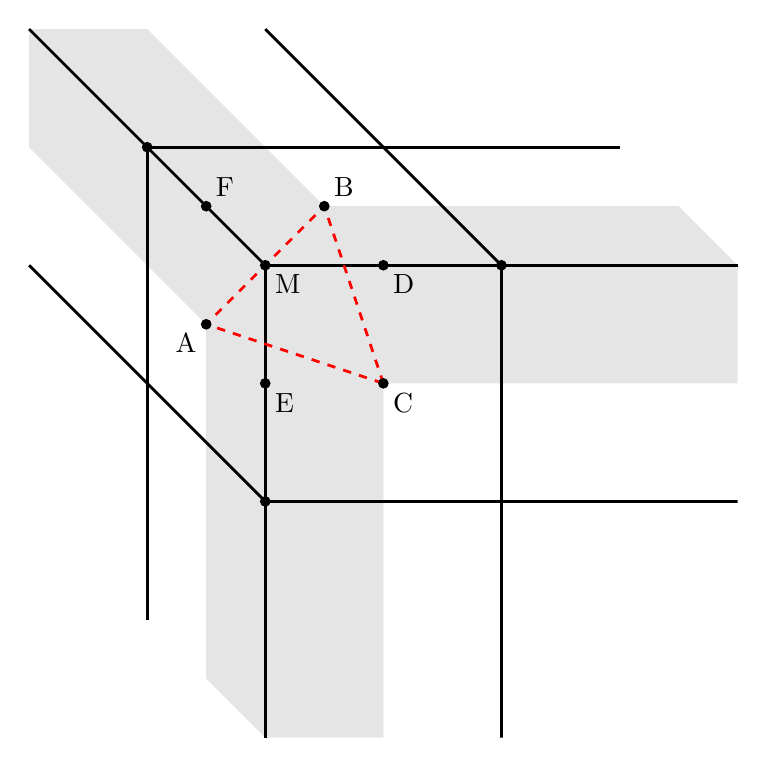
\begin{tikzpicture}[scale=1.5]
\coordinate[] (A) at (0,0);
\coordinate[] (B) at (2,0);
\coordinate[] (C) at (4,0);
\coordinate[] (D) at (0,-2);
\coordinate[] (E) at (2, -2);
\coordinate[] (F) at (4,-2);
\coordinate[] (G) at (0, -4);
\coordinate[] (H) at (2, -4);
\coordinate[] (I) at (4,-4);
\coordinate[] (J) at (-1, 1);
\coordinate[] (K) at (-2, 2);
\coordinate[] (L) at (1, 1);
\coordinate[] (M) at (3, 1);
\coordinate[] (N) at (-1, -1);
\coordinate[] (O) at (-2, 0);
\coordinate[] (P) at (-1, -3);
\coordinate[] (Q) at (-2, -2);
\coordinate[] (R) at (0, 2);
\coordinate[] (S) at (1, -1);
\coordinate[] (T) at (0.5, 0.5);
\coordinate[] (U) at (-0.5, -0.5);
\coordinate[] (V) at (0, -1);
\coordinate[] (W) at (1, 0);
\coordinate[] (Z) at (-0.5, 0.5);
\coordinate[] (A1) at (-2, 1);
\coordinate[] (B1) at (-1, 2);
\coordinate[] (C1) at (3.5, 0.5);
\coordinate[] (D1) at (4, -1);
\coordinate[] (E1) at (1, -4);
\coordinate[] (F1) at (-0.5, -3.5);

\fill [fill=gray!20] (K)--(A1)--(U)--(F1)--(G)--(E1)--(S)--(D1)--(C)--(C1)--(T)--(B1)--cycle;
\draw [line width=1pt] (A) -- (K);
\draw [line width=1pt] (A) -- (C);
\draw [line width=1pt] (A) -- (G);
\draw [line width=1pt] (P) -- (J) -- (M);
\draw [line width=1pt] (O) -- (D) -- (F);
\draw [line width=1pt] (R) -- (B) -- (H);
\draw [line width=1pt,red,dashed] (S) --(T) -- (U) -- cycle;
\draw[anchor=north west] (S) node {C};
\draw[anchor=south west] (T) node {B};
\draw[anchor=north east] (U) node {A};
\draw[anchor=north west] (A) node {M};
\draw[anchor=north west] (W) node {D};
\draw[anchor=north west] (V) node {E};
\draw[anchor=south west] (Z) node {F};
\foreach \p in {A,S,T,U,J,D,B,V,W,Z}
	\fill[fill=black,draw=black,thick] (\p) circle (1.0pt);
\end{tikzpicture}
\endgroup
\end{document}
